\documentclass[10pt]{beamer}

\usetheme[progressbar=frametitle]{metropolis}
\usepackage{appendixnumberbeamer}

\usepackage{booktabs}
\usepackage[scale=2]{ccicons}

\usepackage{pgfplots}
\usepgfplotslibrary{dateplot}


\usepackage{xspace}
\newcommand{\themename}{\textbf{\textsc{metropolis}}\xspace}

\title{Desenvolvimento de um coprocessador de vídeo em FPGA para integração com o Robot Operating System - ROS}
\subtitle{Universidade Federal da Bahia\\
            Programa de Pós-Graduação em Engenharia Elétrica}
\date{\today}
\date{Orientador: Prof. Dr. Wagner Luiz Alves de Oliveira\\Coorientador: Prof. Dr. Paulo César Farias}
\author{Autor: Nestor Dias Pereira Neto}
\institute{Salvador, 5 de dezembro de 2022}
\titlegraphic{\hfill
\includegraphics[height=1.85cm]{imagens/logo.png}}





\begin{document}

\maketitle

\begin{frame}{Agenda}
  \setbeamertemplate{section in toc}[sections numbered]
  \tableofcontents[hideallsubsections]
\end{frame}


%=================================================================
% PROBLEMA
%=================================================================
\section{Introdução}

% Slide 
%-----------------------------------------------------------------
{
\metroset{titleformat frame=smallcaps}
\begin{frame}[fragile]{Problema}
    \begin{itemize}
      \item ROS um pseudo sistema operacional para robótica.
      
      \item Proporciona reutilização de um grande número de nós já desenvolvidos e testados por terceiros.
      
      \item Pode-se criar novos sistemas completos apenas gerenciando esses nós na rede interna do ROS.
      
      \item O número de pacotes para o ROS cresceu em uma taxa muito rápida, desde o ano de seu lançamento, 2007, até 2012 o ROS aumentou de 1 para 3699 pacotes.
    \end{itemize}

 \nocite{LwIP,freertosbook,ROSeffect,PDSfpga,NiosIIbook,ROSfpga}
\end{frame}
}

% Slide 
%-----------------------------------------------------------------
{
\metroset{titleformat frame=smallcaps}
\begin{frame}[fragile]{Problema}
\begin{itemize}
    \item Com a distribuição de tarefas através de vários nós, pode-se criar sistemas cada vez mais complexos, apenas inserindo novos nós na rede ROS.
  
   \item ROS Master tem a função de ser um servidor de nome e serviços para o restante dos nós. Ele identifica os nós na rede.
\end{itemize}
  
\end{frame}
}

% Slide 
%-----------------------------------------------------------------
{
\metroset{titleformat frame=smallcaps}
\begin{frame}[fragile]{Problema}

\begin{figure}[h]
	\caption{ROS Master}
	\begin{center}
		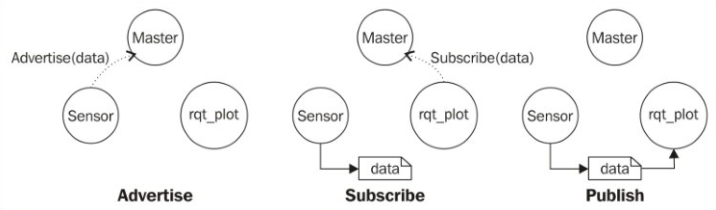
\includegraphics[scale=0.71]{rosMaster.png}\\
		{\small \textbf{Fonte:}\cite{ROSeffect}}
\end{center}
\label{fig:rosmaster}
\end{figure}

\end{frame}
}

% Slide 
%-----------------------------------------------------------------
{
\metroset{titleformat frame=smallcaps}
\begin{frame}[fragile]{Problema}
    \begin{itemize}
        \item Por se tratar de um hardware configurável o FPGA é ideal para processamento digitais de sinais.
        \item O FPGA está próximos a revolucionar o processamento digital de sinais, assim como os DSPs fizeram algumas décadas atrás.
        \item As facilidade de desenvolvimento encontradas em aplicações que fazem uso de softwares não são encontradas nas mesmas proporções no mundo do hardware.
    \end{itemize}
\end{frame}
}


% Slide 
%-----------------------------------------------------------------
{
\metroset{titleformat frame=smallcaps}
\begin{frame}[fragile]{Problema}
	\begin{itemize}
		\item \textbf{Como estabelecer a comunicação entre o ROS e um sistema de processamento de vídeo embarcado em um FPGA? }
	\end{itemize}
	\begin{itemize}
		\item \textbf{O estabelecimento da comunicação entre o FPGA e o ROS e a execução do processamento de vídeo de forma paralela, embarcada em um FPGA, pode melhorar o desempenho do sistema?}
	\end{itemize}
\end{frame}
}


% Slide JUSTIFICATIVA
%-----------------------------------------------------------------
\begin{frame}[fragile]{Justificativa}
    \begin{itemize}
        \item Nos últimos anos, novas técnicas para construção de robôs têm sido bastante estudadas e a robótica móvel tem recebido grande atenção.
        \item Busca por maior autonomia, sistemais mais complexos.
        \item FPGA uma opção para aumento de desempenho computacional, combinado com baixo consumo.
        \item Poucas pesquisas relacionadas ao tema.
        \item Reaproveitamento da pesquisa em outros projetos das mais diversas áreas.
    \end{itemize}
\end{frame}




% Slide OBJETIVOS
%-----------------------------------------------------------------
\subsection{Objetivos}
{
\metroset{titleformat frame=smallcaps}
\begin{frame}{Objetivos}
    \begin{alertblock}{Objetivo geral}
    	\begin{itemize}
    	\item Desenvolver uma solução para estabelecer comunicação entre \textit{Field-Programmable Gate Array - FPGA}, configurado como um coprocessador de vídeo e o \textit{Robot Operating System - ROS}, avaliando o impacto desta aplicação ao sistema.
    	\end{itemize}
    \end{alertblock}
\end{frame}
}




{
\metroset{titleformat frame=smallcaps}
\begin{frame}{Objetivos}
	\begin{alertblock}{Objetivos específicos}
        \begin{itemize}
        	\item Estudar os assuntos relevantes ao projeto: Verilog HDL, RTOS, Nios II, TCO/IP Stack, ROS.
        	\item Conhecer com detalhes os protocolos da rede TCP/IP usada para comunicação interna dos nós e serviços ROS.
        	\item Desenvolver plataforma com Nios II como base para o andamento do projeto.
        	\item Implementar um sistema operacional de tempo real - RTOS na plataforma base.
        	\item Estabelecer comunicação entre o ROS e o sistema Nios II (embarcado no FPGA) através da tecnologia Gigabit Ethernet.
        	\item Testar aplicações de processamento de vídeo em hardware em conjunto com ROS.
        	\item Avaliar a desempenho com a inclusão do FPGA ao sistema.
        \end{itemize}
	\end{alertblock}
\end{frame}
}

%=================================================================
% HIPÓTESE
%=================================================================
\section{Parte I: Referenciais Teórico}
{
\metroset{titleformat frame=smallcaps}
\begin{frame}{Hipótese}
	Para alcançar o objetivo desta pesquisa será necessário desenvolver um sistema, configurado em FPGA, que seja capaz de conectar-se a uma rede TCP/IP. O sistema contará com:
	\begin{itemize}
		\item Soft processor Nios II;
		\item Sistema operacional de tempo real - RTOS;
		\item Biblioteca TCP/IP stack.
	\end{itemize}

\end{frame}
}





%=================================================================
% JUSTIFICATIVA
%=================================================================



%=================================================================
% Metodologia
%=================================================================

\section{Parte II: Desenvolvimento}

\begin{frame}{Metodologia}
    \begin{alertblock}{Procedimentos Metodológicos}
        A pesquisa será realizada em duas fases:
        %\metroset{block=fill}
        \begin{block}{Primeira fase:}
            \begin{itemize}
                \item Levantamento de informações teóricas sobre as tecnologias relacionadas com o tema.
            \end{itemize}
        \end{block}
    
        \begin{block}{Segunda fase}
            \begin{itemize}
                \item Serão desenvolvidos procedimentos, técnicas, algoritmos, circuitos e de todos os procedimentos práticos necessários para alcançar o objetivo da pesquisa.
            \end{itemize}
        \end{block}
    \end{alertblock}

  
\end{frame}

{
\metroset{titleformat frame=smallcaps}
\begin{frame}{Metodologia}
	\begin{alertblock}{Plano de trabalho}
	    \begin{itemize}
	        \item Será apresentado com detalhes nas metas físicas na seção cronograma.
	    \end{itemize}
	\end{alertblock}
	
	\begin{alertblock}{Materiais e infra-estrutura disponível}
	    \begin{itemize}
	        \item Para desenvolvimento do trabalho será utilizado o kit de desenvolvimento DE2-115
        da Terasic, que conta com um FPGA Intel EP4CE115 da família Cyclone IV. Inicialmente
        os teste com o ROS serão no ambiente de simulação Gazebo.
        \end{itemize}
	\end{alertblock}
	
\end{frame}
}

{
\metroset{titleformat frame=smallcaps}
\begin{frame}{Metodologia}
	\begin{alertblock}{Matérias cursadas}
	Todos os créditos obrigatórios com disciplinas já foram concluídos.
	    \begin{itemize}
	        \item Processamento Digitais de Sinais (PPGESP IFBA).
	        \item Processadores Digitais de Sinais - 8,5.
	        \item Inteligência Artificial - 8,0.
	        \item Robótica Móvel - 9,5.
	        \item Processamento Estatístico de Sinais - 8,4.
	        \item Componentes de Processadores Digitais de Sinais - 8,1.
	    \end{itemize}
	\end{alertblock}
	
\end{frame}
}

{
\metroset{titleformat frame=smallcaps}
\begin{frame}{Metodologia}
	\begin{alertblock}{Atividades desenvolvidas}
	Algumas atividades já foram concluídas.
	    \begin{itemize}
	        \item Revisão bibliográfica, estudo de trabalhos relacionado.
	        \item Conhecimento das ferramentas utilizadas.
	        \item Testes com sistema Nios II.
	        \item Implementação do FreeRTOS no NiosII.
	    \end{itemize}
	\end{alertblock}
	
\end{frame}
}


%=================================================================
% Cronograma
%=================================================================

\section{Parte III: Resultados}

{
\metroset{titleformat frame=smallcaps}
\begin{frame}{Cronograma}
	\begin{alertblock}{Metas físicas}
        \begin{enumerate}
        	\item Levantamento bibliográfico sobre os assuntos mais relevantes do projeto: ROS, Nios II, Verilog HDL, RTOS, TCP/IP Stack, Sockets.
        	\item Estudo detalhado do protocolo de comunicação entre os nós no ROS.
        	\item Desenvolvimento do sistema base do Nios II no Platform Designer.
        	\item Implementação do RTOS no sistema base.
        	\item Testes de comunicação TCP/IP entre o PC e o sistema embarcado no FPGA.
        	\item Desenvolvimento de uma aplicação de processamento de vídeo em FPGA.
        	\item Avaliação do desempenho do sistema proposto.
        	\item Elaboração da dissertação e publicação dos resultados.
        \end{enumerate}
	\end{alertblock}
\end{frame}
}

{
\metroset{titleformat frame=smallcaps}
\begin{frame}{Cronograma}

    \begin{table}[h]
    	\centering

    	\vspace{0.2cm}
    	\begin{tabular}{c|cccccccccccc}
    		\toprule
    		 & \multicolumn{12}{c}{{\tiny Meses}}\\ 
    		{\tiny Metas} & {\tiny 1} & {\tiny 2} & {\tiny 3} & {\tiny 4} & {\tiny 5} & {\tiny 6} & {\tiny 7} & {\tiny 8} & {\tiny 9} & {\tiny 10} & {\tiny 11} & {\tiny 12} \\ 
    		\midrule  
    		\midrule                           
    		{\tiny Levantamento Bibliográfico}& $\circledast$ & & & & & & & & & & & \\
    		\hline
    		{\tiny Estudo protocolos ROS} & & $\circledast$ & $\circledast$ & $\circledast$ & $\circledast$ & $\circledast$ & & & & & &  \\
    		\hline
    		{\tiny Desenv. do Nios II} & & & $\circledast$ & $\circledast$ & & & & & & & &  \\
    		\hline
    		{\tiny Implementação } {\tiny do RTOS} & & & & $\circledast$ & $\circledast$ & $\circledast$ & & & & & &  \\
    		\hline
    		{\tiny Testes de Comunicação} & & & & & & $\circledast$ & $\circledast$ & $\circledast$ & & & &  \\
    		\hline
    		{\tiny Desenv. do coprocessador} & & & & & & & & $\circledast$ & $\circledast$ & $\circledast$ & $\circledast$ &  \\
    		\hline
    		{\tiny Avaliação do desempenho} & & & & & & & & & & $\circledast$ & $\circledast$ & $\circledast$ \\
    		\hline
    		{\tiny Elaboração da } {\tiny dissertação} & & & & & & $\circledast$ & $\circledast$ & $\circledast$ & $\circledast$ & $\circledast$ & $\circledast$ & $\circledast$\\
    		\bottomrule 
    
    	\end{tabular}
    	\\
    	\label{tab:crono}
    \end{table}
\end{frame}
}

%{\setbeamercolor{palette primary}{fg=black, bg=yellow}
%\begin{frame}[standout]
%  Questions?
%\end{frame}
%}


\begin{frame}[allowframebreaks]{Referencias}

  \bibliography{demo}
  %\bibliographystyle{abbrv}
  \bibliographystyle{acm}
  
\end{frame}

\end{document}



%\begin{frame}{Blocks}
%  Three different block environments are pre-defined and may be styled with an
%  optional background color.

%  \begin{columns}[T,onlytextwidth]
%    \column{0.5\textwidth}
%      \begin{block}{Default}
%        Block content.
%      \end{block}

%      \begin{alertblock}{Alert}
%        Block content.
%      \end{alertblock}

%      \begin{exampleblock}{Example}
%        Block content.
%      \end{exampleblock}

%    \column{0.5\textwidth}

%      \metroset{block=fill}

%      \begin{block}{Default}
%        Block content.
%      \end{block}

%      \begin{alertblock}{Alert}
%        Block content.
%      \end{alertblock}

%      \begin{exampleblock}{Example}
%        Block content.
%      \end{exampleblock}
%
%  \end{columns}
%\end{frame}




%{%
%\setbeamertemplate{frame footer}{My custom footer}
%\begin{frame}[fragile]{Frame footer}
%    \themename defines a custom beamer template to add a text to the footer. It can be set via
%    \begin{verbatim}\setbeamertemplate{frame footer}{My custom footer}\end{verbatim}
%\end{frame}
%}